\section{The camera gimbal}
A gimbal is device which can rotate about one or more axis \cite{website:definition_gimbal}. A typical use is to place a camera and 3 actuators on a gimbal, resulting in the ability to rotate the camera in the roll, pitch and yaw axis. An annotated render of this can be found in Figure~\ref{fig:roll_pitch_yaw_camera}.

\begin{figure}[h!]
  \centering
  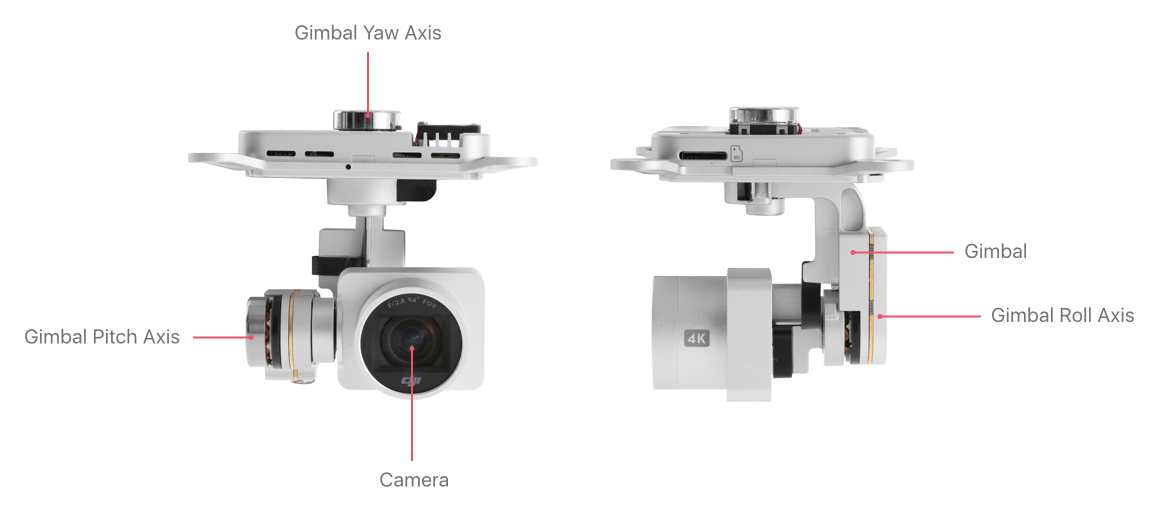
\includegraphics[width=\textwidth]{literature_review/roll_pitch_yaw_gimbal.png}
  \caption{\label{fig:roll_pitch_yaw_camera} An illustration of the roll, pitch and yaw axis used in a gimbal~\cite{roll_pitch_yaw_camera}.}
\end{figure}

While gimbal designs are \emph{fairly} standard, a few critical design choices must be made when building or buying one.% The rest of this chapter will detail some of the options available.

\subsection{Comparison of actuator types}
The type of actuator used in the gimbal has a significant effect on the design of the gimbal (due to actuator shape), the speed it can move, the camera weight it can handle and quality of the resulting photos and videos (due to actuator vibrations). Thus, three relevant actuator types (a brushed DC motor, a servomotor and a BLDC motor) were considered and compared, taking into account the selection available at local stores.

%\begin{table}[h!]
%	\centering
%	\begin{tabular}{ p{2cm}||p{4cm}|p{4cm}|p{4cm} }
%					& DC motor			& Servo motor		& BLDC \\
%	\hline \hline
%	Length			& $\approx 45mm$	& $\approx 50mm$	& $<30mm$ \\
%	\hline
%	Diameter		& $\approx 30mm$	& $50mm\times 20mm$	& $<30mm$ \\
%	\hline
%	Weight			& Moderate			& Heavier			& Light, requires ESC \\
%	\hline
%	Complexity		& Moderate (H-bridge) & Simple (built in) & Difficult (requires PID controller) \\
%	\hline
%	Circuitry required & H-bridge		& None (built in)	& Requires ESCs \\
%	\hline
%	Efficiency		& Low				& Low				& High \\
%	\hline
%	Maximum speed	& Low				& Low				& High \\
%	\hline
%	Price			& Low/moderate		& Low/moderate		& High \\
%	\hline
%	Smoothness		& Moderate			& Low				& Very high \\
%	\hline
%	\end{tabular}
%	\caption{Comparison of gimbal actuators}
%	\label{table:gimbal_actuators}
%\end{table}

%To summarize the main highlights from table \ref{table:gimbal_actuators}:

To make the comparison more concrete, specific possible models were chosen. The DC (Direct Current) motor considered was 99:1 Metal Gearmotor available from Pololu.com \cite{DC_motor_choice}. The servo motor was a 20kg.cm Metal Gear Servo available from Robotics.org.za \cite{servo_motor_choice}. Finally, the Brushless DC (BLDC) motor was a Quanum 2208 brushless gimbal motor \cite{bldc_motor_choice} available second hand.

The DC motor is relatively long and heavy. It also requires an additional H-bridge circuit to drive it. Finally, it wasn't clear how the Raspberry Pi (running a non realtime OS) would use the rotational decoder and apply a control law.

The servo motor is relatively easy to use as the Raspberry Pi has built in PWM. It also has relatively high torque. However, it too is relatively large and would likely move in a jittery fashion, resulting in lower quality footage.

Lastly, the BLDC motor is potentially expensive and quite complex to use. Its advantages are its was compactness, low weight and high speed. It is worth noting that, while controlling BLDC motors can be fairly complex, using a store-bought controller allows for one to easily leverage off the design work of other engineers. This results in a faster, smoother and more stable gimbal than one could build in a short period of time.

\subsection{\label{ssec:gimbal_design_inspirations}Gimbal design inspirations}
It is useful to review existing gimbal designs in order to avoid unnecessary re-invention of the wheel. Luckily, a large number of designs are available on the internet. One design which stood out from the research phase was \href{https://www.thingiverse.com}{thingiverse.com} member Velocirotor's clever gimbal design, dubbed the \href{https://www.thingiverse.com/thing:2804872}{Primbal Session} \cite{website:primbal_session}. It is light-weight, simple to 3D print and has an easy method to adjust length to balance the gimbal's three axis. A render of the design can be found in Figure~\ref{fig:primbal_pic}.

\begin{figure}[h!]
  \centering
  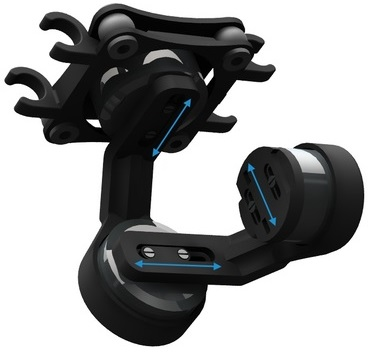
\includegraphics[width=0.7\textwidth]{literature_review/primbal_pic.jpg}
  \caption{\label{fig:primbal_pic} A render of the Primbal Session gimbal design.}
\end{figure}

Some inspiration was also taken from a gimbal designed by mechatronics engineering student Sylvan Morris, made during a period of vacation work. Noteworthy characteristics include the two-plate shock absorption system and method of mounting onto a quadcopter. A photo of his design can be found in Figure~\ref{fig:sylvan_gimbal}.

\begin{figure}[ht!]
  \centering
  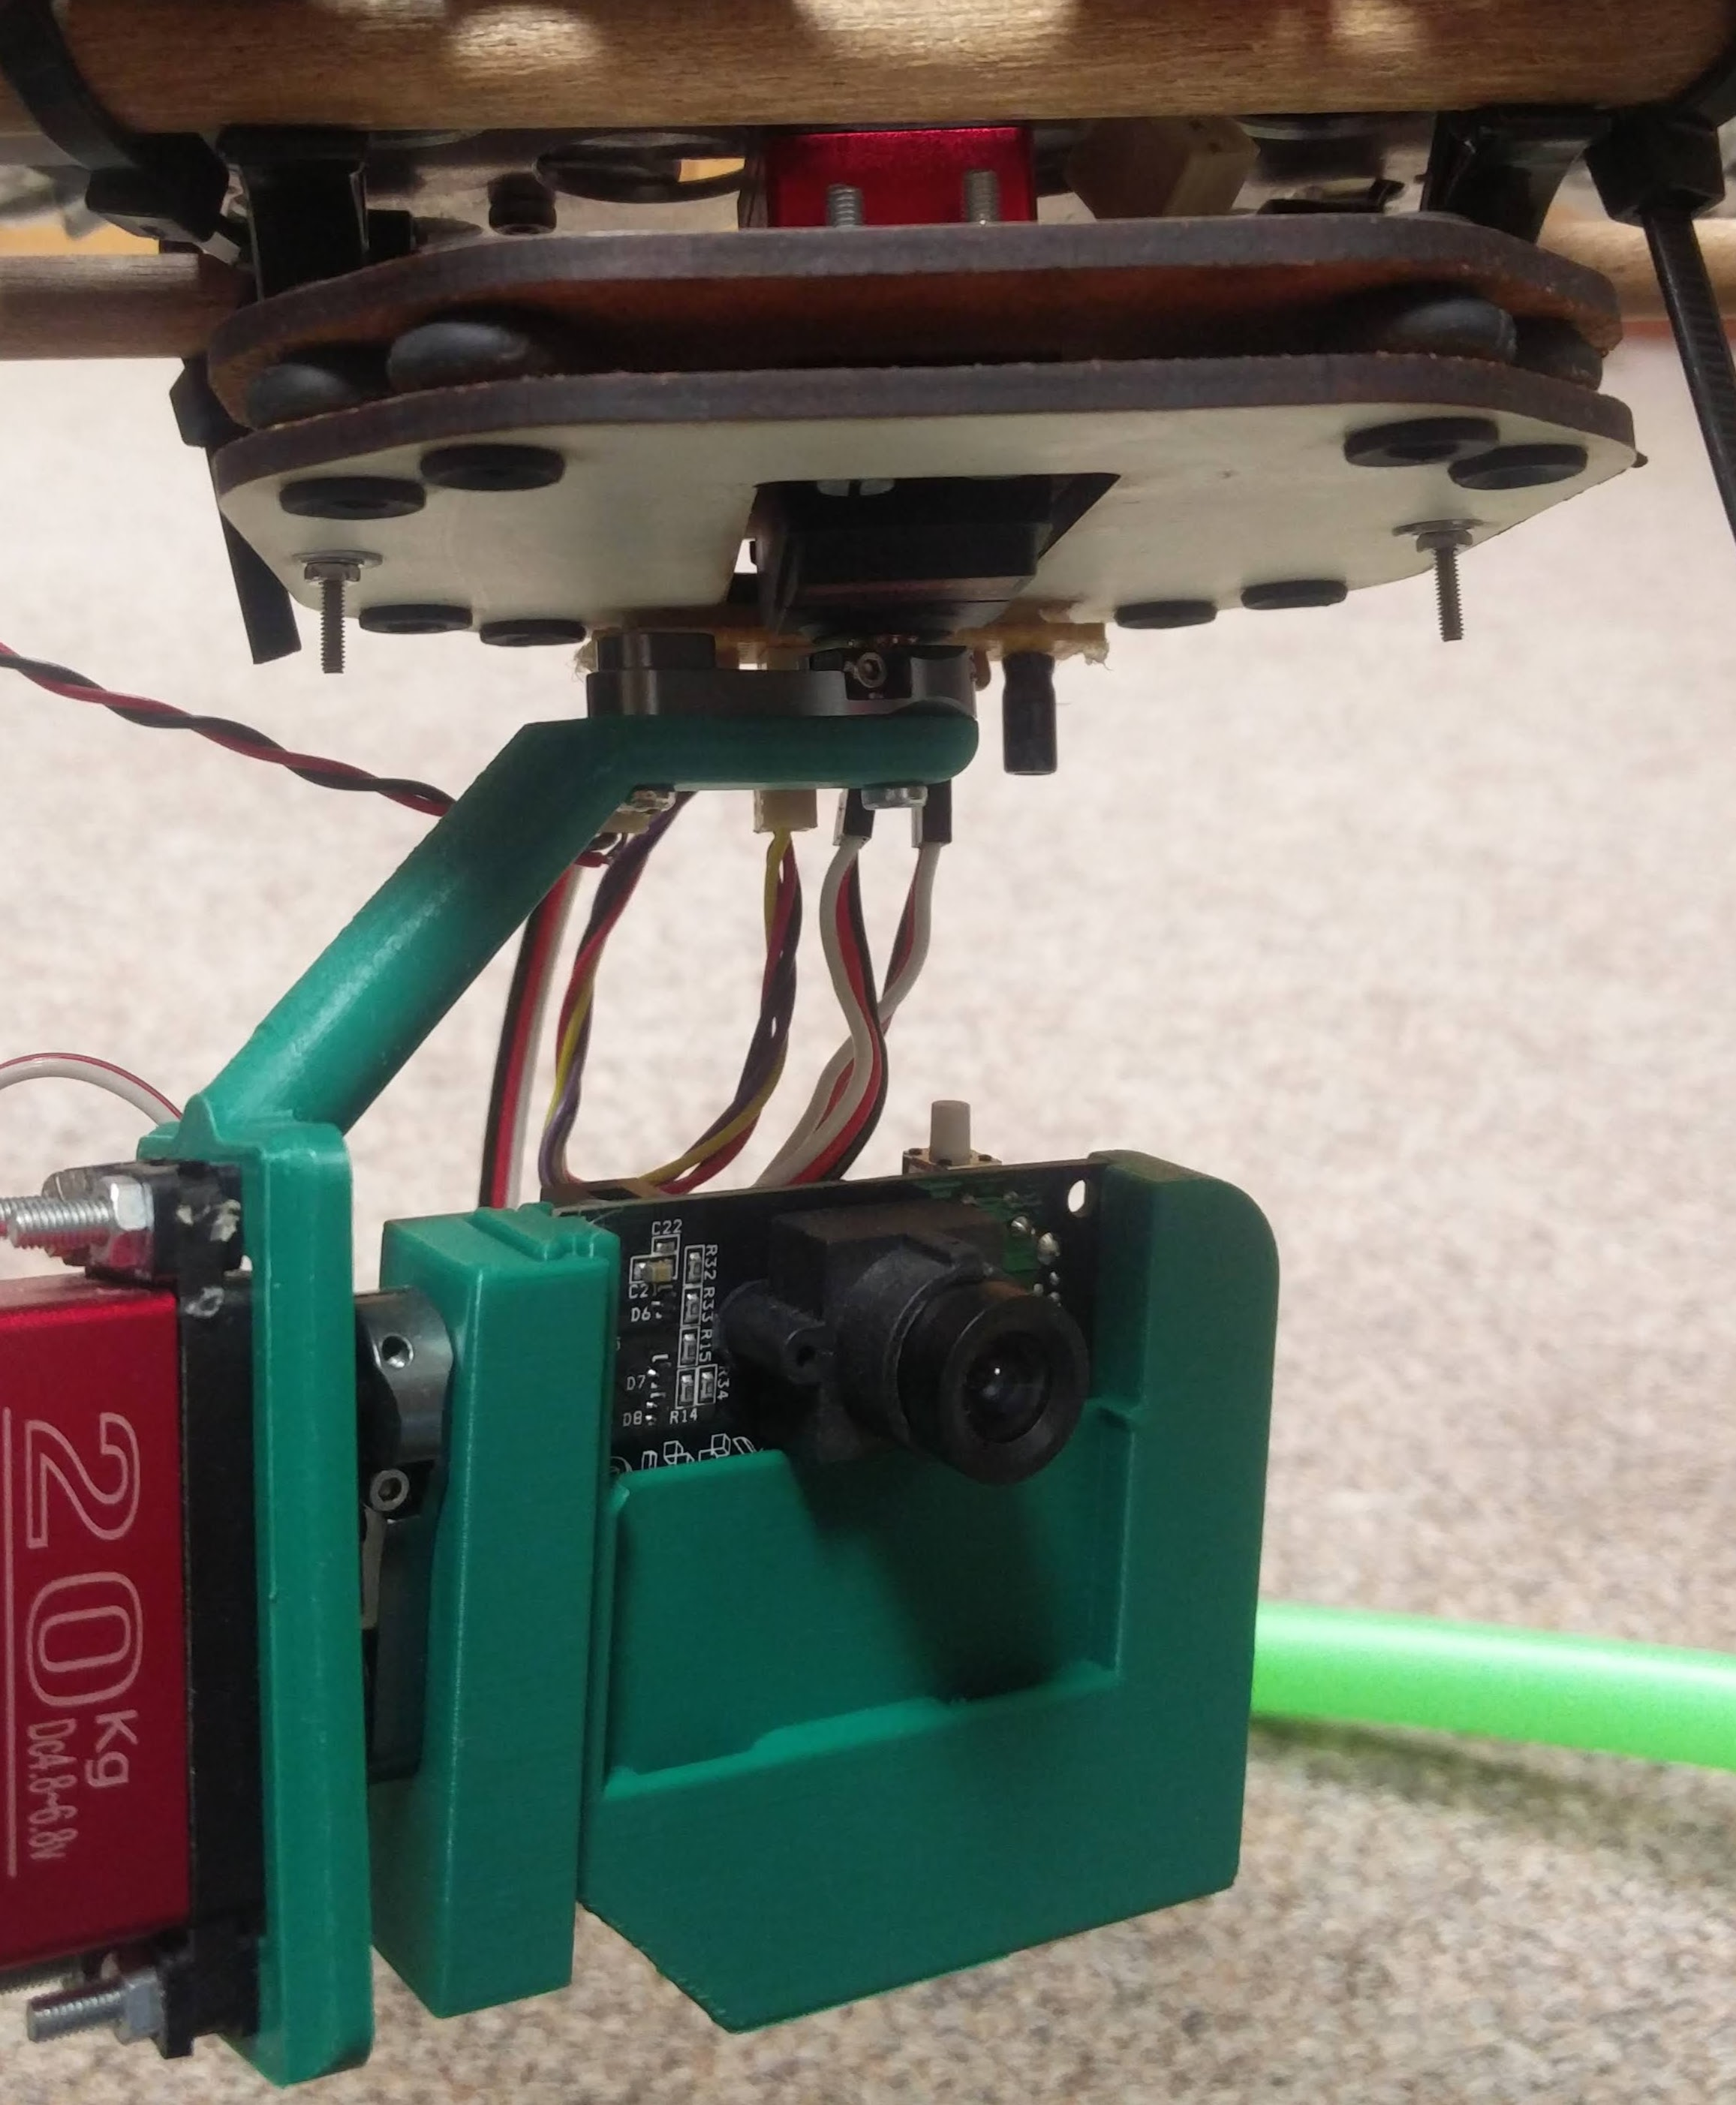
\includegraphics[width=0.7\textwidth]{literature_review/sylvan_gimbal.jpg}
  \caption{\label{fig:sylvan_gimbal} A photo of Sylvan Morris's gimbal design.}
\end{figure}

